\chapter{OUTPUT}
\begin{spacing}{1.5}
The screenshots of the prototype program developed. The entire source code is available in GitHub - {\it https://github.com/abilng/sMash.it}

\begin{figure}
        \centering
        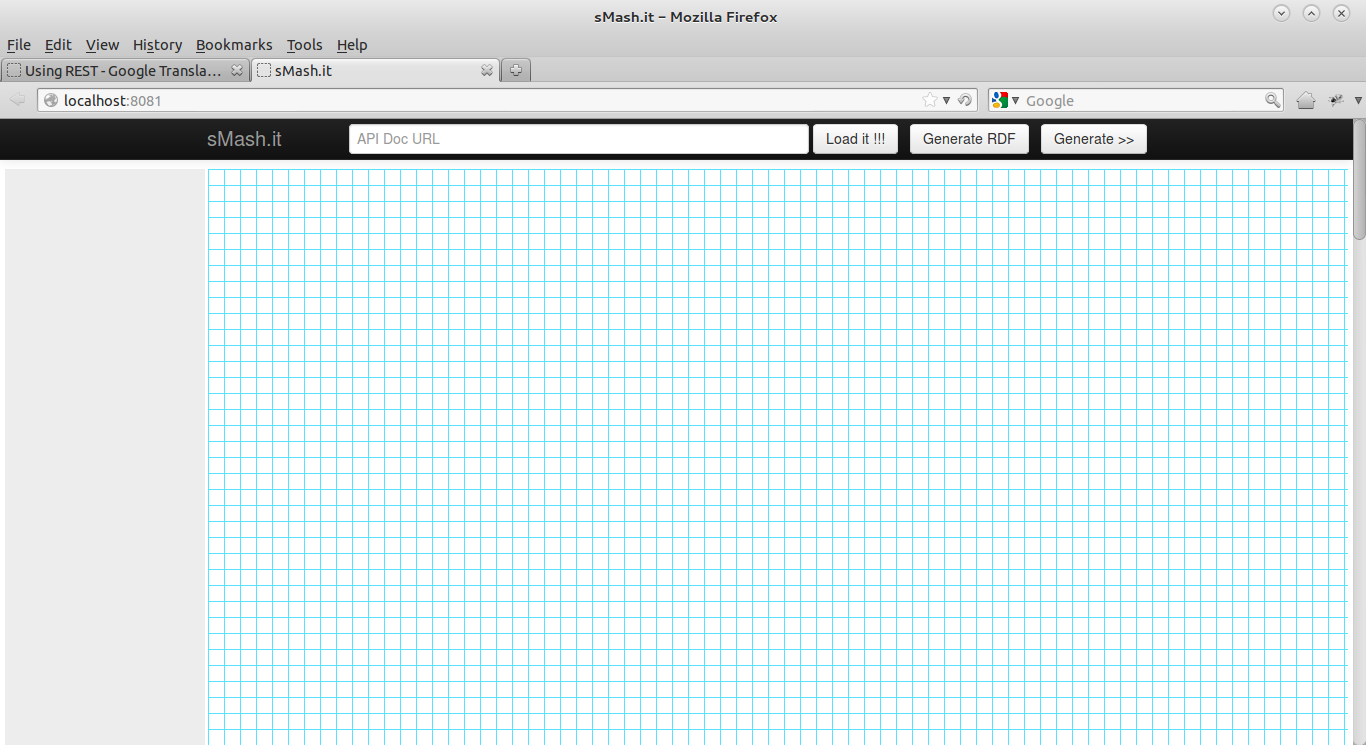
\includegraphics[scale=0.3]{images/7.png}
        \caption{Client Homescreen and workbench}
\end{figure}

\begin{figure}
        \centering
        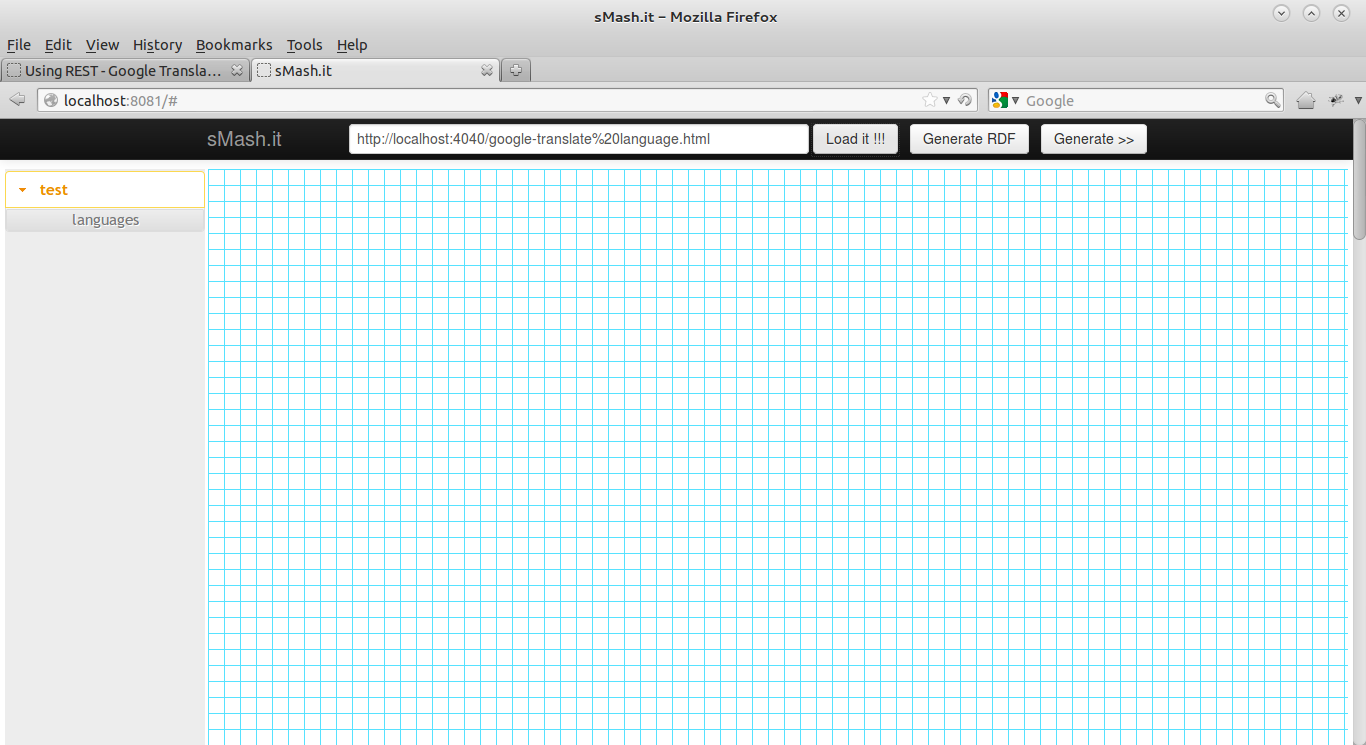
\includegraphics[scale=0.3]{images/6.png}
        \caption{Loading an API}
\end{figure}


\begin{figure}
        \centering
        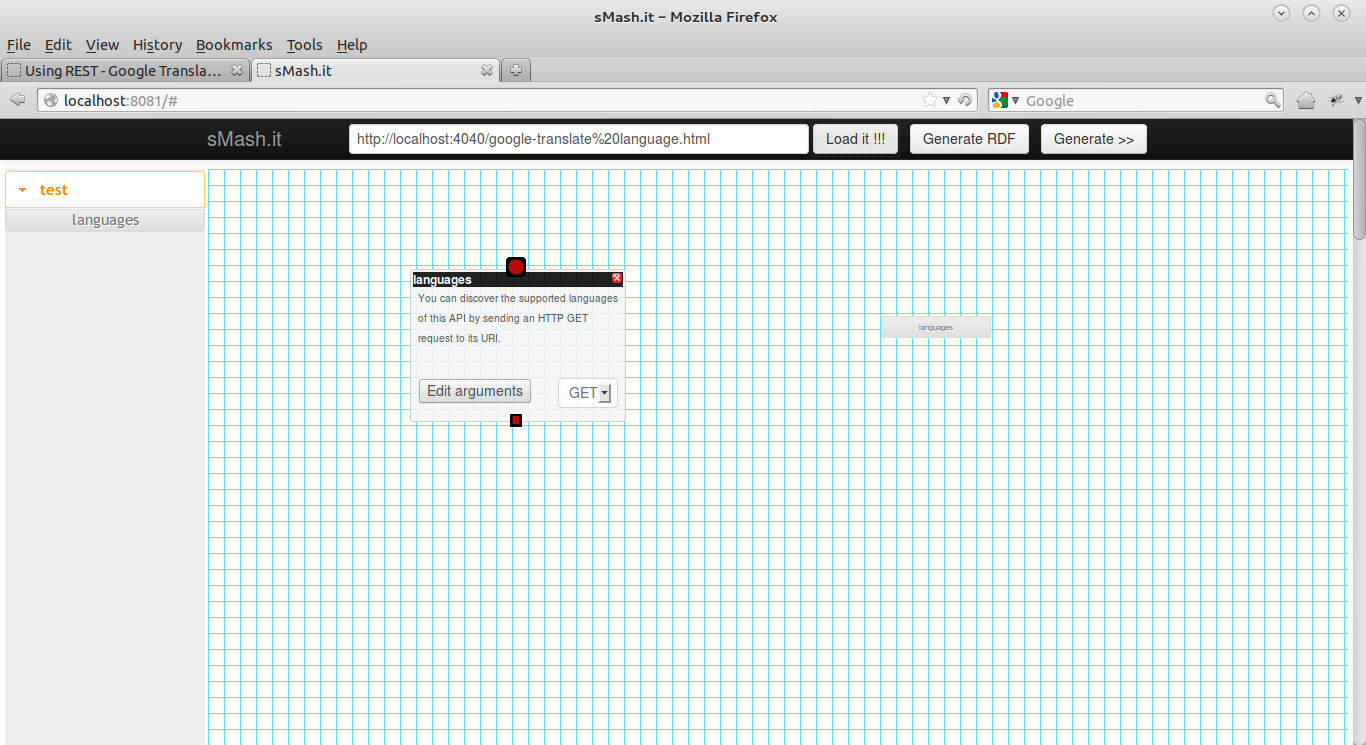
\includegraphics[scale=0.3]{images/5.png}
        \caption{Mashup design using drag n drop - step 1}
\end{figure}

\begin{figure}
        \centering
        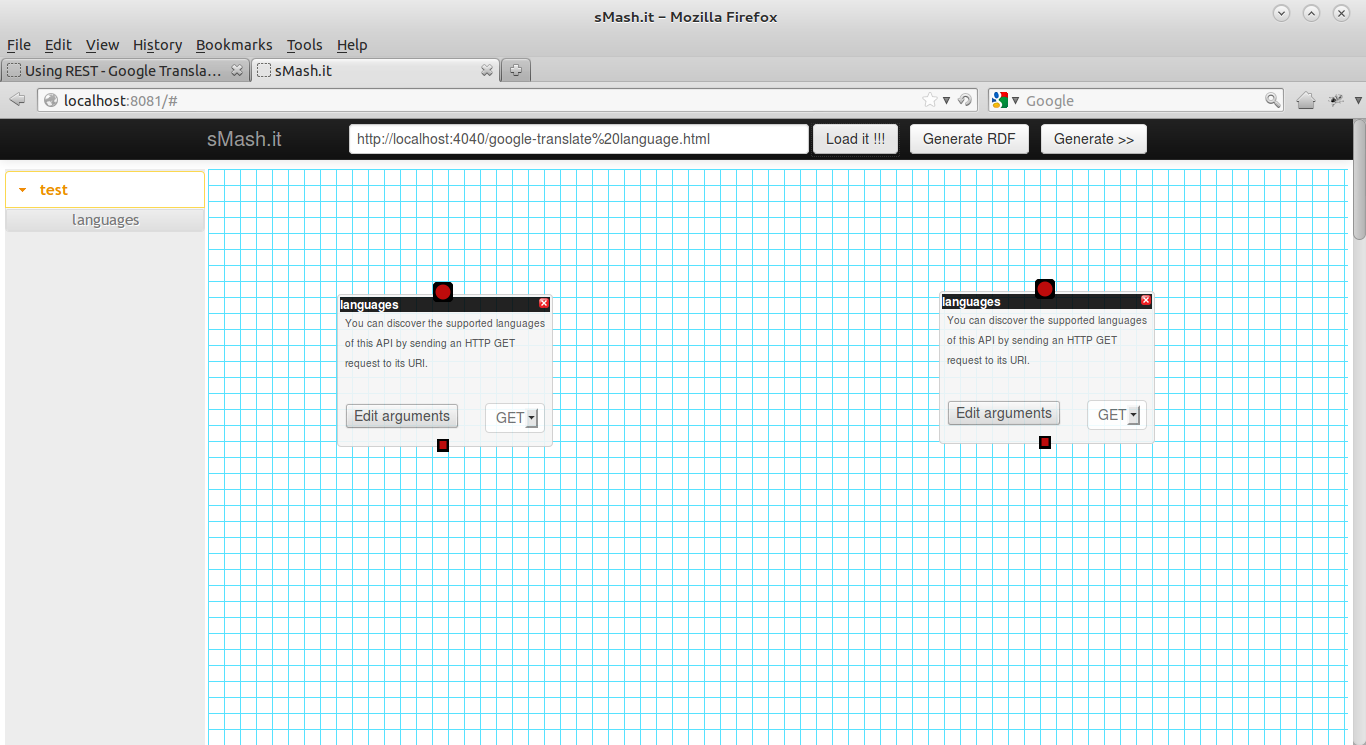
\includegraphics[scale=0.3]{images/4.png}
        \caption{Mashup design using drag n drop -step 2}
\end{figure}


\begin{figure}
        \centering
        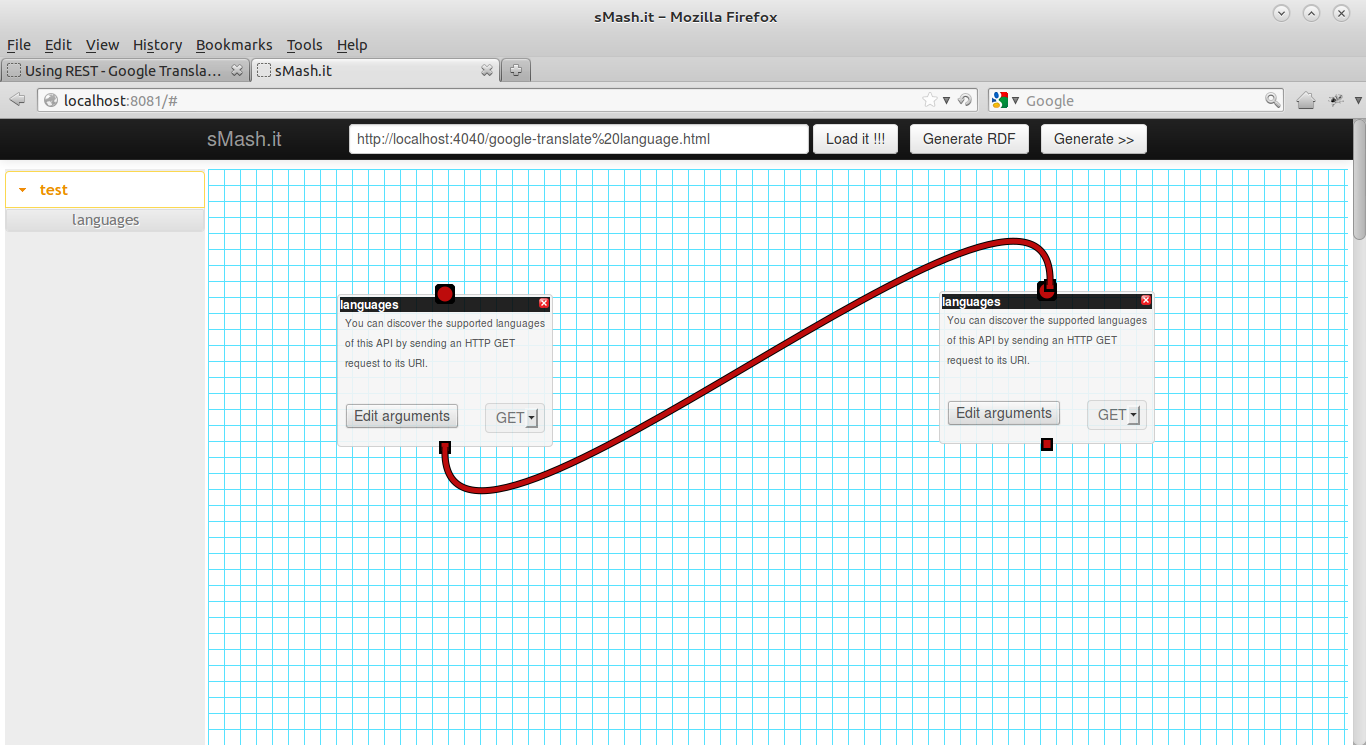
\includegraphics[scale=0.3]{images/3.png}
        \caption{Mashup design using drag n drop -step 3}
\end{figure}


\begin{figure}
        \centering
        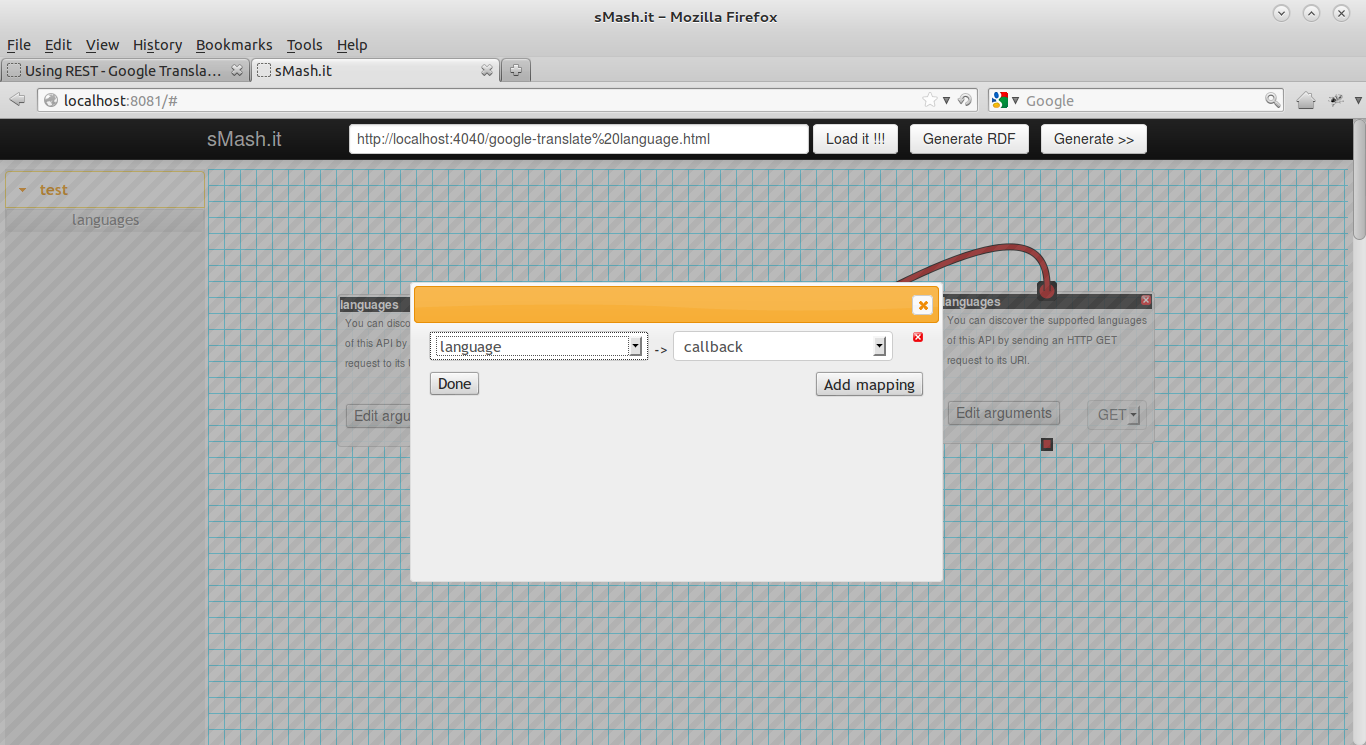
\includegraphics[scale=0.3]{images/2.png}
        \caption{Mashup creation-step 4, Parameter mapping.}
\end{figure}

\begin{figure}
        \centering
        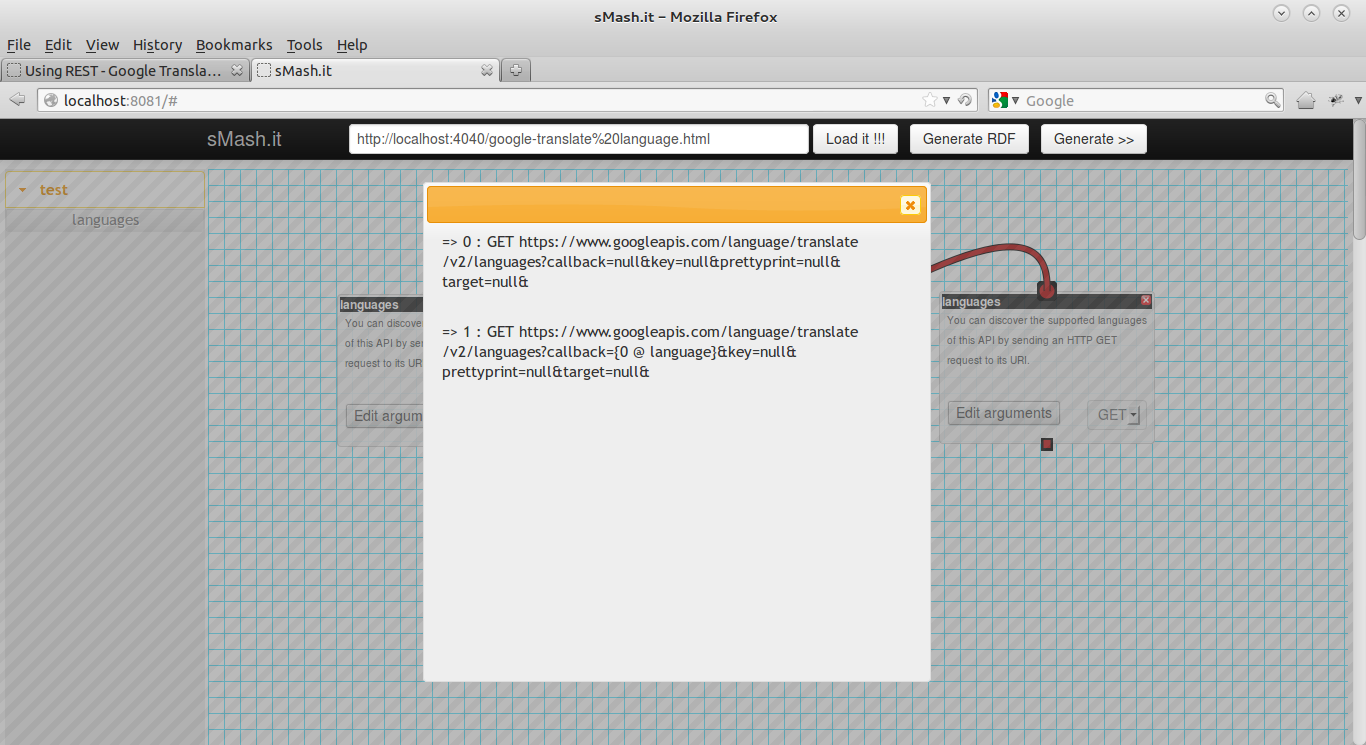
\includegraphics[scale=0.3]{images/1.png}
        \caption{Invocation sequence generated.}
\end{figure}
\end{spacing}